\documentclass[a4paper,12pt]{article}
\usepackage[english]{babel}
\usepackage[utf8]{inputenc}

%
% For alternative styles, see the biblatex manual:
% http://mirrors.ctan.org/macros/latex/contrib/biblatex/doc/biblatex.pdf
%
% The 'verbose' family of styles produces full citations in footnotes, 
% with and a variety of options for ibidem abbreviations.
%
\usepackage{graphicx}
\usepackage{csquotes}
\usepackage[style=verbose-ibid,backend=bibtex]{biblatex}
\bibliography{sample}

\usepackage{lipsum} % for dummy text

\title{The Linear Programming Approach to Approximate Dynamic Programming}

\author{Shayan Amani}

\date{\today}

\begin{document}
\maketitle

\section{Intro}
Authors in this paper have tried to come up with a way to approximate cost-to-go function ($J$) with a set of "basis functions" ($\phi$). In terms of approximation, they finally showed that the proposed generalization over the linear programming (LP) approach could conform to the solution which dynamic programming (DP) gives us. The motivation for picking an LP solution over DP is in tight relation to two criteria, first one, on the one hand, is barely clear understanding about the way that DP works under the hood and on the other hand, scarce in references for implementation of DP is the second reason that they claim to be a motivation to prefer LP over DP.

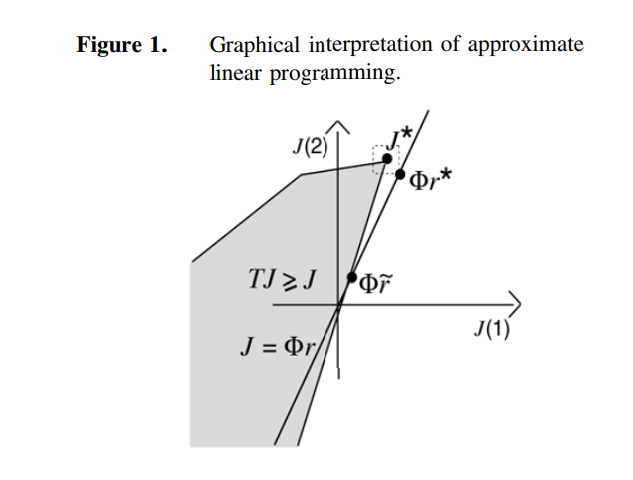
\includegraphics[width=1\columnwidth]{alp-fig.png}


In order to eliminating the gigantic set of state spaces in real-world problems which leads to sparsity (A.K.A \textit{curse of dimensionality}), this solution can help in a considerable amount to shrink the state space down with taking advantage of basis-functions and generally the approximation techniques introduced here.

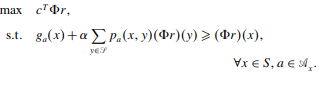
\includegraphics[width=1\columnwidth]{lp.png}

\section{Questions}
\subsection{ If the optimal value function is one of the features, will ALP compute the optimal value function?}
According to the Theorem 2:

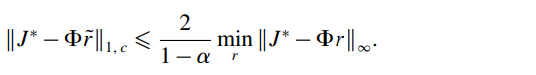
\includegraphics[width=1\columnwidth]{alp-theorem2.png}

we can realize that ALP always yields a solution which falls in the bounded criterion no matter which set of features you pass into it.

\subsection{How does the computational complexity of ALP compare to LSPI? Which one is better?}
The major portion of computation work in ALP is turning around the way that the method approximate cost function with basis-function features. In a huge problem with a massive (and sparse at the same time) state space, solving the problem using ALP is preferable in terms of computation efficiency and that is because of picking a shrunk down set of features.

% This is an example citation \autocite{ginsberg}.
% \lipsum[1] % dummy text

% This is another example citation \autocite{brassard}.
% \lipsum[2] % dummy text

% This is a repeated citation \autocite{brassard}.
% \lipsum[3] % dummy text

% This is another example citation \autocite{adorf}.
% \lipsum[4] % dummy text 

\end{document}